\subsection{QR Code \& Indoor Localization}

As we discussed previously, GPS is not the right choice when it comes to indoor localization, and we even mentioned some of the other replacements. But since we want to develop a system that exploits the information rich visuals using a camera, we can use this camera to detect QR Codes and determining the user's precise position as we are going to mention in more details at the methodology section.

There are several useful and interesting ways of determining the user's position after detecting and decoding a QR Code. One way for example, is dividing the environment into several squares, each square has its own QR Code inside of it encoding its position, whether it is put on the floor, roof, wall, or even in a hanging panel from the roof. For better illustration, let us assume that we have a room of 4 meters in width and height, this room is divided into 16 squares with equal sizes so each square has an area of 1m$^2$. If we customized a hat for example, that embeds a camera in its top, the user's position will get determined while navigating in the room wearing the hat. 

\begin{figure}[h]
	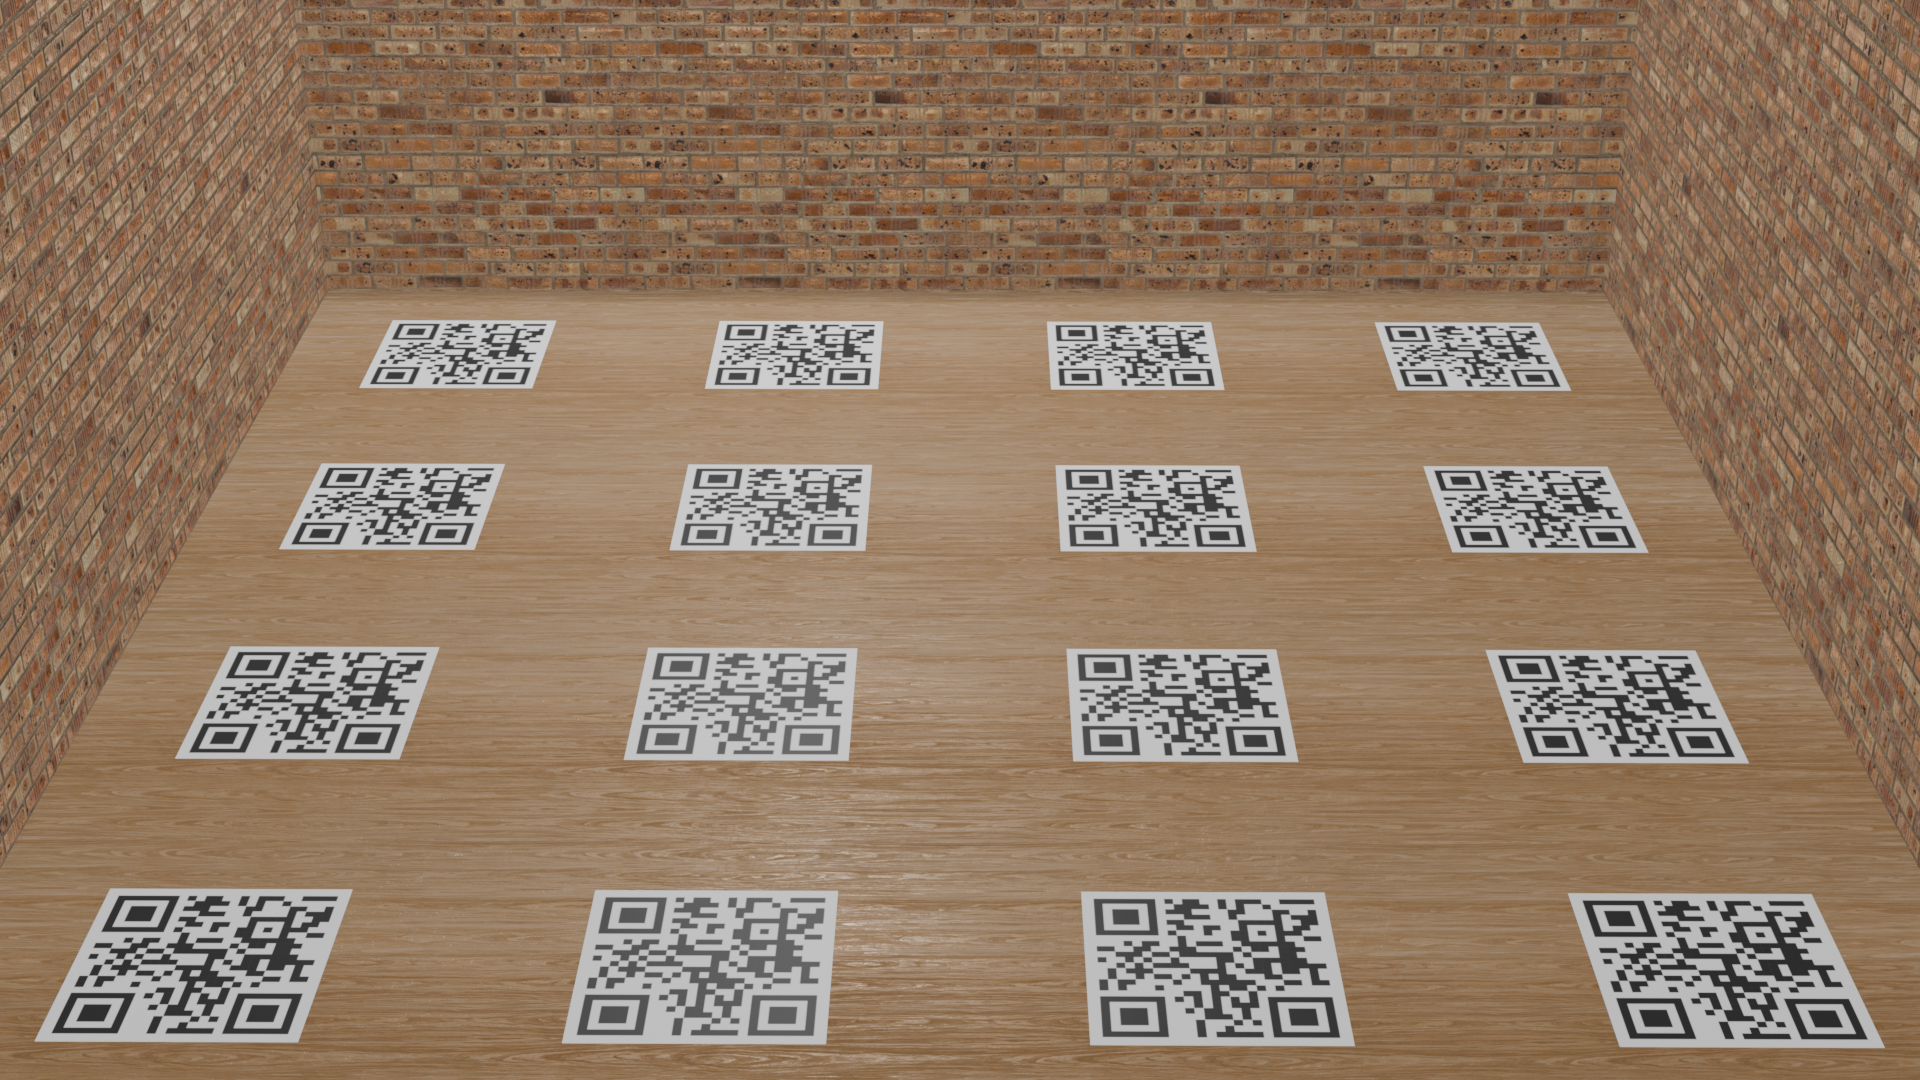
\includegraphics[width=\textwidth]{assets/ch2/Divided room for QR Codes/Divided room for QR Codes.png}
	\caption{ This image illustrates how a room can be divided into squares each with its own QR Code. }
\end{figure}

Although this solution is very computationally cheap, it comes with its own downsides. For instance, the position values are always discrete. So if we needed a continuous and precise position we should not use this method. But actually, this method could be very useful depending on its use. See [3] for example, where they created a localization system for a robot by assigning a QR Code for each floor tile/block, and they also assigned some tiles as obstacles so the robot will avoid trying to move on them. Then they used Dijkstra’s algorithm so the robot can find the shortest path from its current node to any other node.

\color{purple}
The idea of dividing an environment into smaller pieces is widely used in some industries in different ways and purposes. One of these industries is the video game industry. A huge amount of video games divide the game world into a chunk of squares, triangles, hexagons, and other shapes depending on the game's need and performance. But the difference here is that they do not use this technique for localization since the positions for all the objects in the games are known and stored at the RAMs already. They use the technique to categorize the pieces such as walkable ground, water, lava, rocks, and so on. Then these pieces are used along with their categories to find a proper path between two points. Different path finding algorithms can be used, but the most popular and simple one is A* algorithm. See this [4] incredible youtube tutorial made by Sebastian Lague, that explain an implementation of the A* algorithm and how it can be optimized.
\color{black}

Another important and interesting way to calculate a precise and continues values of the user's position is detecting and decoding a QR Code using a camera, then calculating the position and orientation (pose) of it relative to the camera, after that we will be able to use this pose and the QR Code's global position to estimate the user's precise position. This method is heavier at the CPU, and harder to implement. It also need the camera's intrinsic parameters to be known or calculated using camera calibration algorithm. More on details could be found at the methodology section. See [5], where they used this method for implementing their localization system.